\section{Kommunikation}
\label{sec:comm}

Da viele Daten in hoher Frequenz übertragen werden müssen, (Nach jeder Veränderung des Dokuments
muss der Server informiert werden, der dann zu unbestimmten Zeitpunkten in mehreren Schritten die
Zustands- Informationen zurücksendet) ist eine normale Datenübertagung wie bei Webapplikationen
üblich über \acr{ajax} bzw. \acr{http}-Anfragen nicht gut geeignet: Bei normalem \acr{http} ist es
zum einen immer nötig auf Browser Seite eine Anfrage zu stellen um Informationen vom Server zu
erhalten, zum anderen hat jede Anfrage und jede Antwort zusätzlich einen Header, welcher mindestens
einige hundert Bytes groß ist.

Als Worst-Case Beispiel kann das Entfernen von Kommandos aus dem Dokumenten-Modell betrachtet
werden: Um das Modell eines Dokuments auf Server und Client synchron zu halten müssen ab und zu
Nachrichten vom Server gesendet werden, welche signalisieren, dass ein Kommando aus dem Modell
entfernt wurde. Diese Nachricht enthält als Information die eindeutige ID des Kommandos. Bei der ID
handelt es sich um eine 64-Bit Zahl. Zusätzlich dazu muss signalisiert werden, um welche Aktion es
sich eigentlich handelt. Dafür reichen bei der überschaubaren Anzahl an möglichen Aktionen weitere 4
Byte mehr als aus. Das bedeutet, die eigentlichen Informationen die für diese Aktion relevant sind
belaufen sich auf höchstens 12 Byte. Würde diese Aktion über \acr{http} laufen müsste zunächst eine
Anfrage gestellt werden

\begin{lstlisting}
GET /user/project/file.thy/remove-command HTTP/1.1
Host: www.clide.net
\end{lstlisting}

Diese Anfrage allein ist bereits 70 Zeichen lang ohne dass überhaupt relevante Informationen
übertragen wurden. Die minimale Antwort sähe dann in etwa so aus:

\begin{lstlisting}
HTTP/1.1 200 OK
Server: Apache/1.3.29 (Unix) PHP/4.3.4
Content-Length: 12
Content-Language: de
Connection: close
Content-Type: text/html

178
\end{lstlisting}

Das sind zusammen über 250 Zeichen um zu signalisieren, dass Kommando 178 entfernt werden soll.
Damit wurde die Information um den Faktor 30 aufgeblasen. Zusätzlich kommt es zu Verzögerungen durch
die zusätzlichen Anfragen. 

\subsection{WebSockets}
\label{sec:ws}

Die im \acr{html}5-Standard eingeführten WebSockets sind die ideale Lösung für dieses Problem. Bei
WebSockets wird eine vollduplex Verbindung über TCP aufgebaut, welche ohne den HTTP-Overhead
auskommt und lediglich ein Byte pro Nachricht benötigt um zu signalisiern, dass eine Nachricht
endet. Außerdem ist es durch die duplex Verbindung möglich sogenannte Server-Pushes wie in dem
vorangegangenen Beispiel ohne vorheriges Polling bzw. eine verzögerte Antwort auf eine Anfrage zu
realisieren.

Dadurch, dass WebSockets ein relativ neues Konzept bilden, werden durch deren Anwendung die meisten
älteren Browser von der Benutzung der Webapplikation ausgeschlossen. Ein Fallback auf HTTP wäre zwar
relativ leicht zu implementieren, aber in der Benutzung kaum akzeptabel, da sich die zusätzlichen
Verzögerungen bei teilweise weit über 1000 Nachrichten pro Minute so negativ auf die
Ausführungsgeschwindigkeit auswirken würden, dass ein produktives Arbeiten mit dem System nicht mehr
möglich wäre. Aktuell werden WebSockets von allen relevanten Browsern in der neusten Version
unterstützt. Browser die seit einem Jahr nicht mehr aktualisiert wurden können mit dem Aufruf
allerding zu großen Teilen nichts Anfangen. (Siehe \ref{sec:comp}) Das Play-Webframwork unterstützt
Serverseitige WebSocket-Verbindungen. Allerding muss bei der Benutzung auf viel Funktionalität
verzichtet werden. Da WebSockets allerdings so unabdingbar sind werden diese Einschränkungen
akzeptiert.

\begin{figure}[ht]
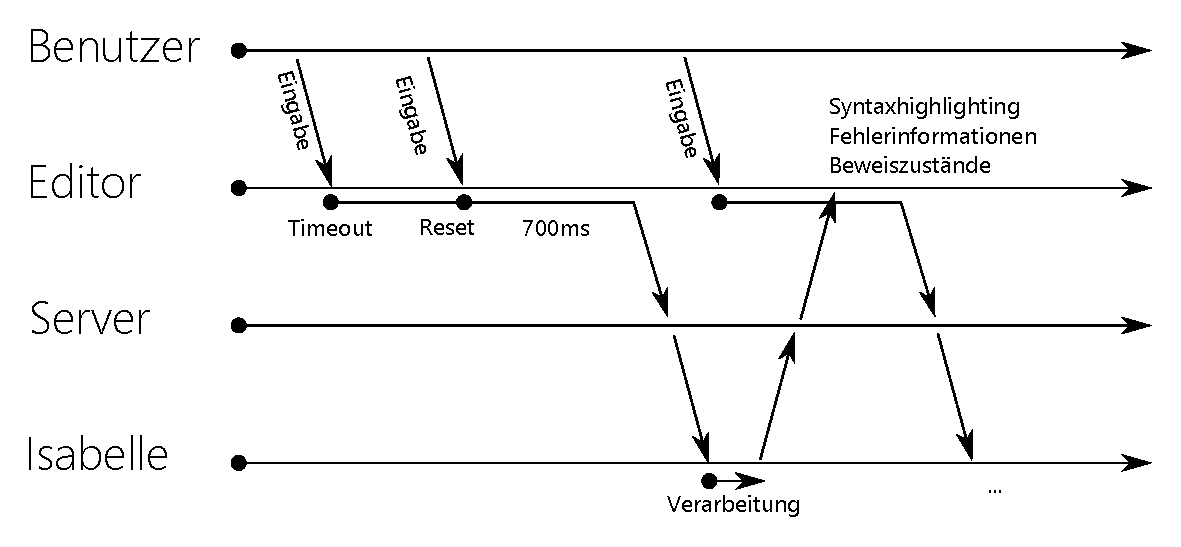
\includegraphics[width=\linewidth]{images/diagram-workflow}
  \caption{Datenfluss in clide}  
  \label{fig:diagram-workflow}
\end{figure}

\subsection{Protokoll}

Für das Protokoll wurde zunächst der Einfachheit halber \acr{json} gewählt mit der Möglichkeit im
Hinterkopf, es zu einem späteren Zeitpunkt leicht duch das komprimierte \acr{bson}-Protokoll zu
ersetzen. Um das möglich zu machen wird unter Verwendung von Dynamischer Typisierung in Scala (Siehe
Abschnitt\ref{sec:dyn}) vom Protokoll abstrahiert, (Siehe Abschnitt \ref{sec:jsc}) damit es das
Übertragungsprotokoll selbst ohne größeren Aufwand ausgetauscht werden kann.

\clearpage